\section{QS-Prozess nach Iteration}
So wie das Projekt ist auch der QS-Prozess im Projektverlauf angewachsen. Es wurden neue Tools hinzugefügt
und neue Testumgebungen entwickelt, da die Auftraggeber ihre Anforderungen geändert haben. Daher gibt
es nicht für alle Iterationen vollständige Testausgaben. Zudem haben einige Tools (AppVeyor und Travis CI)
die gleichen Tests durchgeführt. Dort wurde dann nur ein Output angehängt.

Die Iterationslänge betrug zwei Wochen.

\subsubsection{1. Iteration}
\begin{table}[H]
\begin{center}
	\begin{tabular}{| l | l |}
		\hline
		\textbf{Zeitraum} & 13.11.2017 - 26.11.2017\\\hline
		\textbf{Abgegebene Userstorys} & 1, 2, 6, 14, 15, 16 \\\hline
		\textbf{Commit Hash} & \texttt{f3bbc82b0eb9ef5c0159843152fc54fb7c5c8309} \\\hline
	\end{tabular}
	\caption{Übersicht 1. Iteration}
\end{center}
\end{table}

\subsubsection{Testoutput (\texttt{python manage.py test})}
\lstinputlisting{test_output/01_iteration_python}

\subsubsection{2. Iteration}
\begin{table}[H]
\begin{center}
	\begin{tabular}{| l | l |}
		\hline
		\textbf{Zeitraum} & 27.11.2017 - 10.12.2017\\\hline
		\textbf{Abgegebene Userstorys} & 3, 19, 20, 21\\\hline
		\textbf{Commit Hash} & \texttt{eef5badcf7928d55461bfddb40c3f7f7194a0fa3} \\\hline
	\end{tabular}
	\caption{Übersicht 2. Iteration}
\end{center}
\end{table}
\subsubsection{Testoutput (\texttt{python manage.py test})}
\lstinputlisting{test_output/02_iteration_python}

\subsubsection{3. Iteration}
\begin{table}[H]
\begin{center}
	\begin{tabular}{| l | l |}
		\hline
		\textbf{Zeitraum} & 11.12.2017 - 07.01.2018\\\hline
		\textbf{Abgegebene Userstorys} & 5, 7, 17, 22, 23, 24, 27\\\hline
		\textbf{Commit Hash} & \texttt{b5c84ab3496ade220316b8b119c7fddc3d49d383} \\\hline
	\end{tabular}
	\caption{Übersicht 3. Iteration}
\end{center}
\end{table}
\subsubsection{Testoutput (\texttt{python manage.py test})}
\lstinputlisting{test_output/03_iteration_python}
\subsubsection{Coverage}
\begin{figure}[H]
	\centering
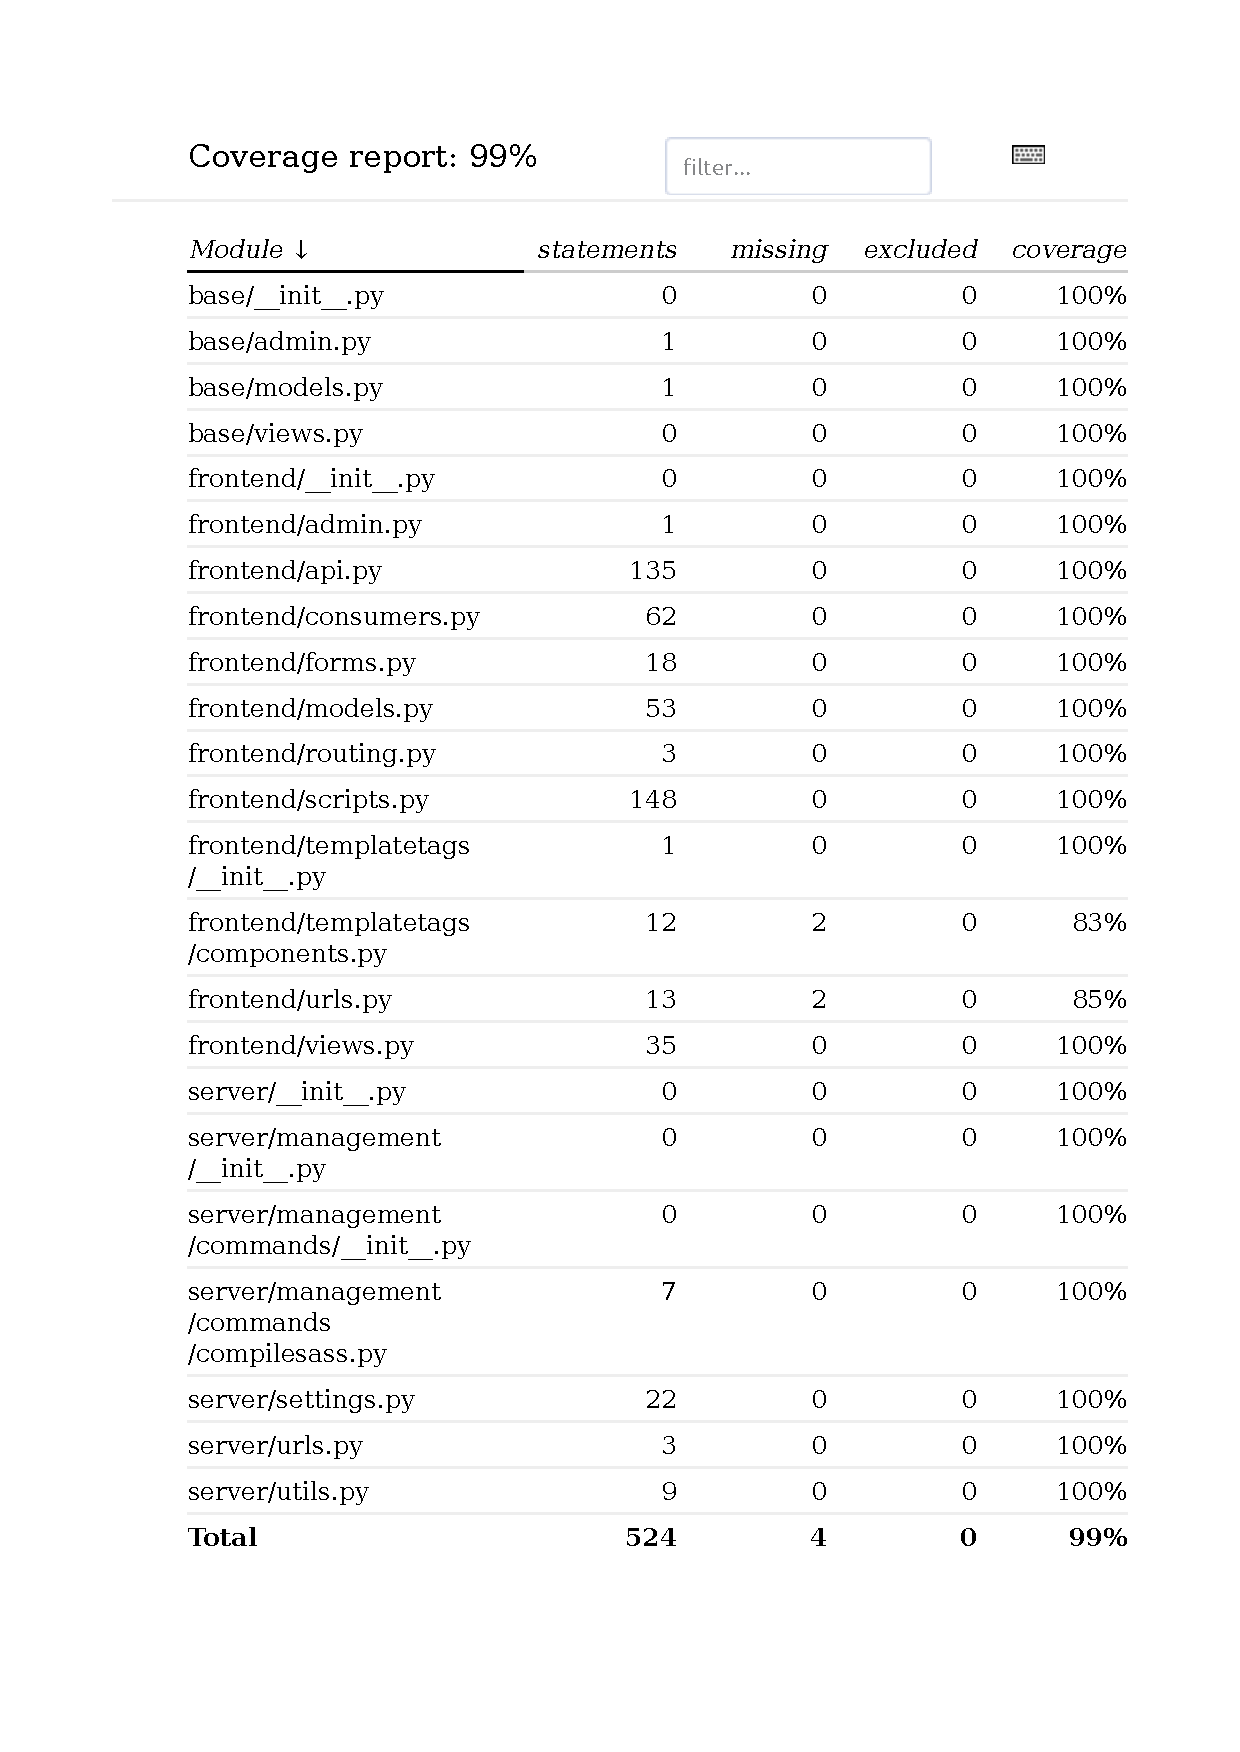
\includegraphics[width=.9\textwidth]{test_output/03_iteration_coverage.pdf}
	\caption{Coverage in Iteration 3}
\end{figure}

\subsubsection{4. Iteration}
\begin{table}[H]
\begin{center}
	\begin{tabular}{| l | l |}
		\hline
		\textbf{Zeitraum} & 08.01.2018 - 21.01.2018\\\hline
		\textbf{Abgegebene Userstorys} & 4, 8, 28, 29, 33, 34, 35, 36, \\\hline
		\textbf{Commit Hash} & \texttt{b06b3f8b23a022a127061c2dae05215c0bc21f23} \\\hline
	\end{tabular}
	\caption{Übersicht 4. Iteration}
\end{center}
\end{table}
\subsubsection{Testoutput (\texttt{python manage.py test})}
\lstinputlisting{test_output/04_iteration_python}
\subsubsection{Coverage}
\begin{figure}[H]
	\centering
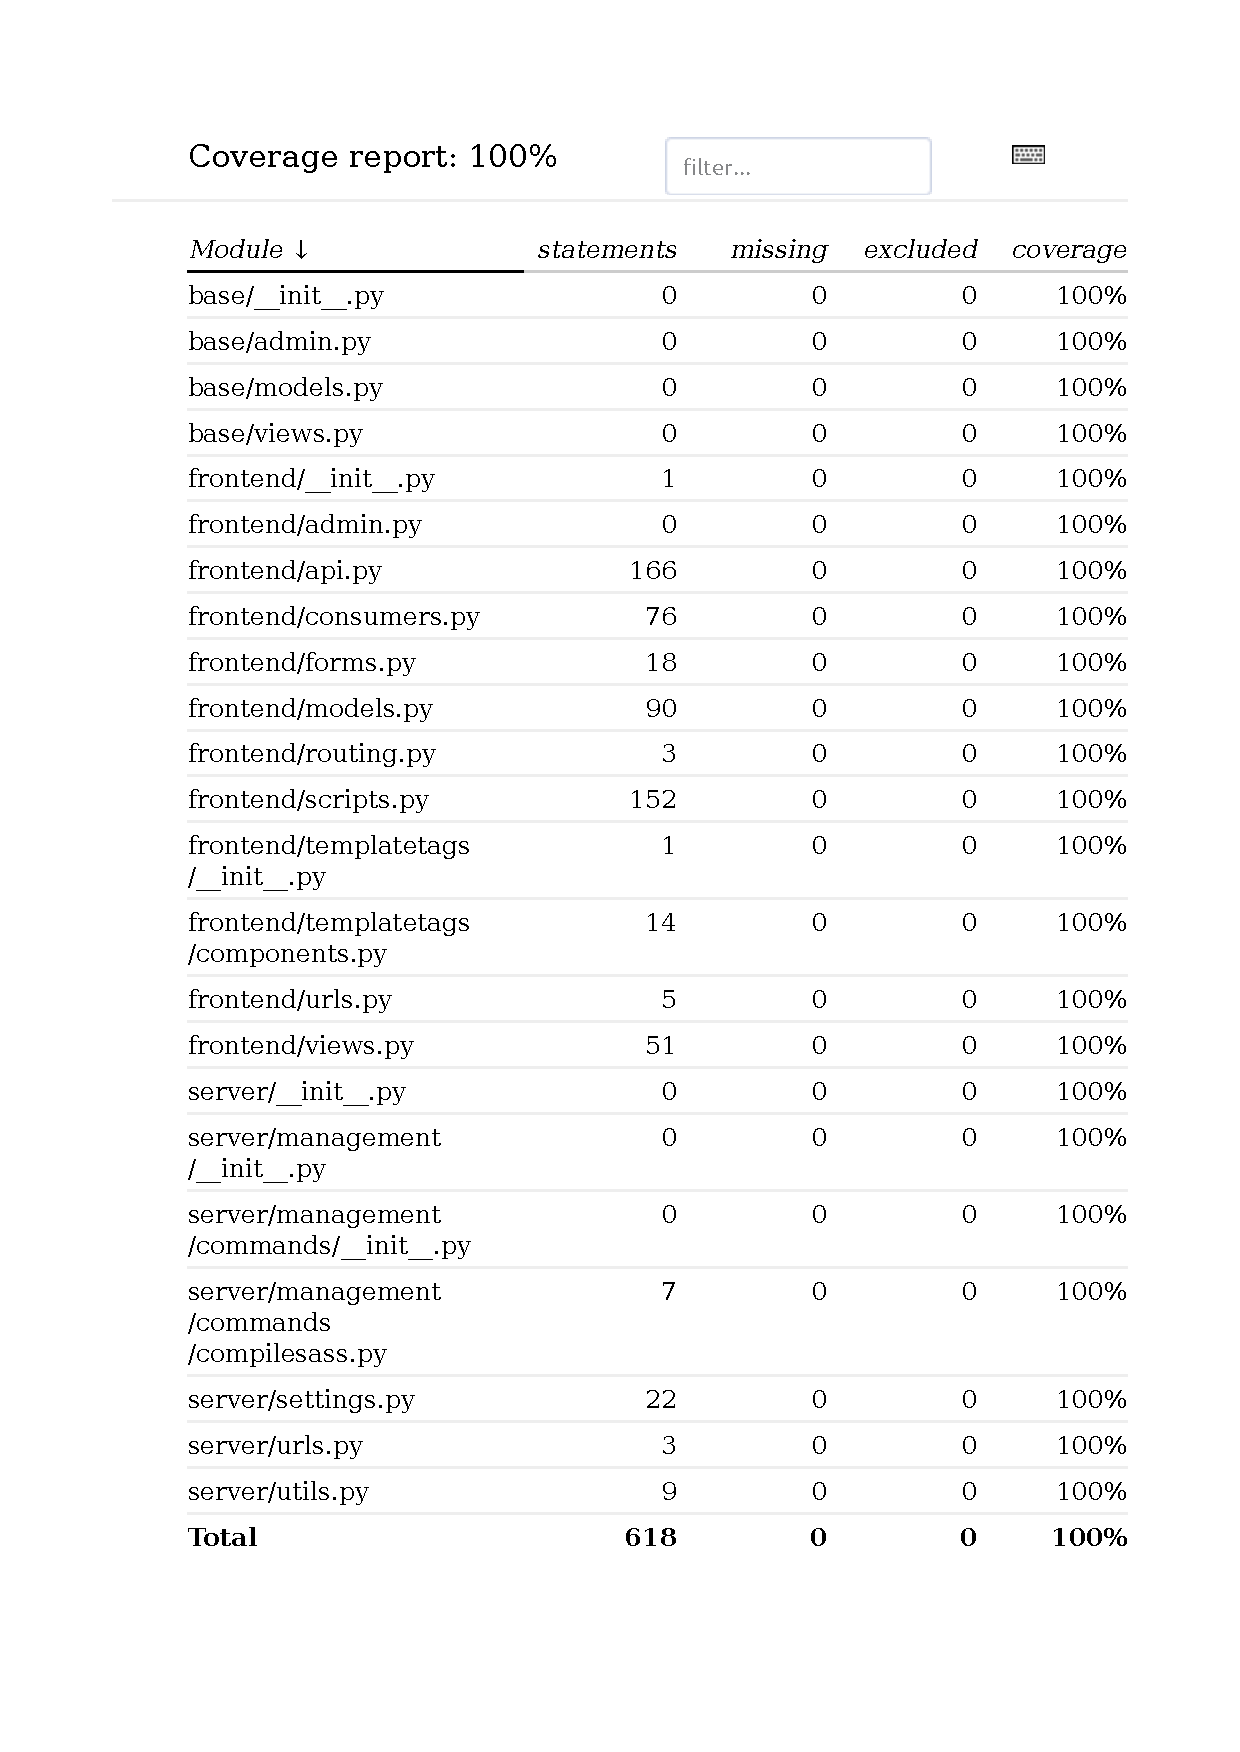
\includegraphics[width=.9\textwidth]{test_output/04_iteration_coverage.pdf}
	\caption{Coverage in Iteration 4}
\end{figure}

\subsubsection{5. Iteration}
\begin{table}[H]
\begin{center}
	\begin{tabular}{| l | l |}
		\hline
		\textbf{Zeitraum} &  22.01.2018 - 04.02.2018\\\hline
		\textbf{Abgegebene Userstorys} & 25, 31\\\hline
		\textbf{Commit Hash} & \texttt{8a194372e807cc043f3ea705671d515fd0fe0bb5} \\\hline
	\end{tabular}
	\caption{Übersicht 5. Iteration}
\end{center}
\end{table}
\subsubsection{Testoutput }
\lstinputlisting{test_output/05_iteration_python}
\subsubsection{Coverage}
\begin{figure}[H]
	\centering
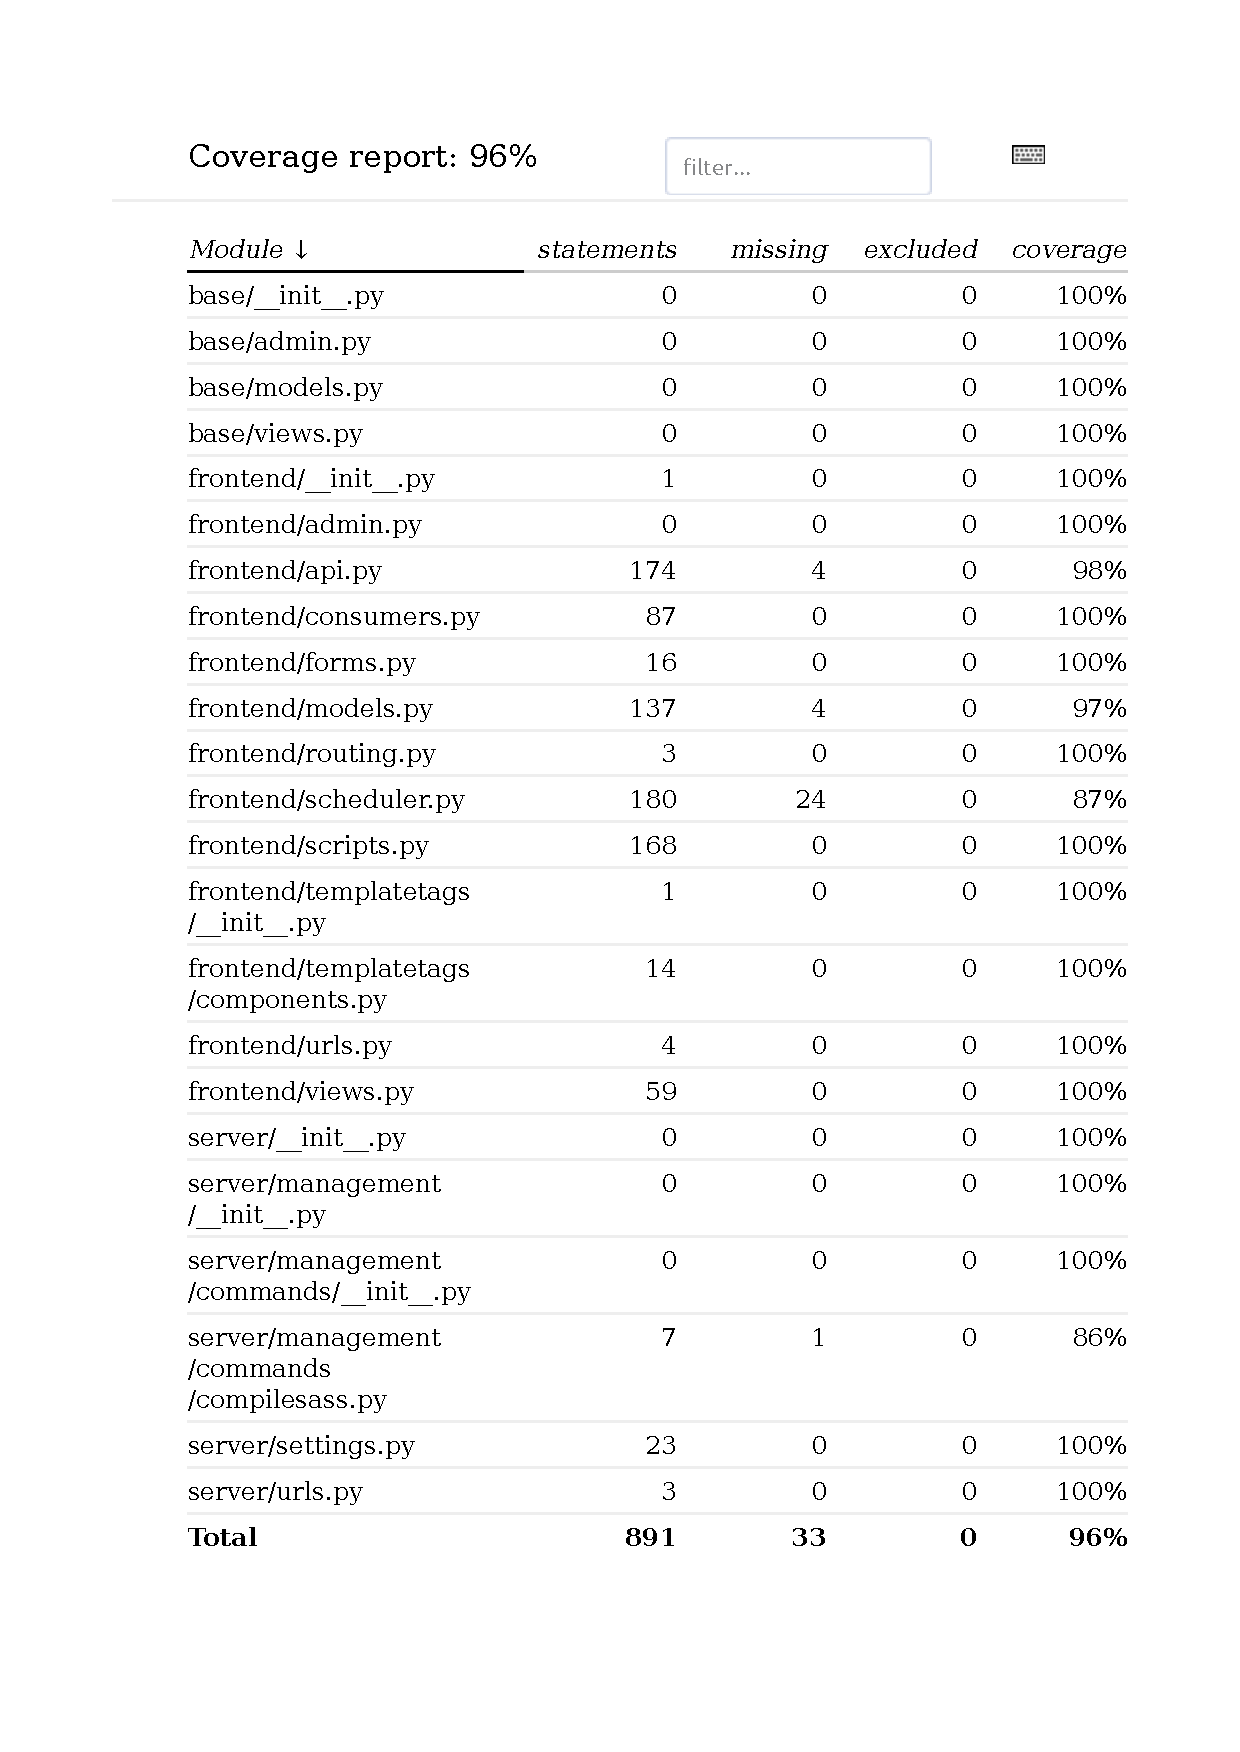
\includegraphics[width=.9\textwidth]{test_output/05_iteration_coverage.pdf}
	\caption{Coverage in Iteration 5}
\end{figure}

\subsubsection{6. Iteration}
\todo[inline]{Erklärung für fehlende Userstorys einfügen}
\begin{table}[H]
\begin{center}
	\begin{tabular}{| l | l |}
		\hline
		\textbf{Zeitraum} &  05.02.2018 - 18.02.2018\\\hline
		\textbf{Abgegebene Userstorys} & EDIT EXPLANATION.mp3 (Keine Us vorhanden)\\\hline
		\textbf{Commit Hash} & \texttt{KEIN COMMIT} \\\hline
	\end{tabular}
	\caption{Übersicht 6. Iteration}
\end{center}
\end{table}

\subsubsection{7. Iteration}
\begin{table}[H]
\begin{center}
	\begin{tabular}{| l | l |}
		\hline
		\textbf{Zeitraum} &  19.02.2018 - 04.03.2018\\\hline
		\textbf{Abgegebene Userstorys} & 9,26,30,37,38,39,40\\\hline
		\textbf{Commit Hash} & \texttt{6003099c26804bff6995ac4ff0d0d5571dfc2840} \\\hline
	\end{tabular}
	\caption{Übersicht 7. Iteration}
\end{center}
\end{table}
\subsubsection{Testoutput }
\lstinputlisting{test_output/07_iteration_python}
\subsubsection{Coverage}
\begin{figure}[H]
	\centering
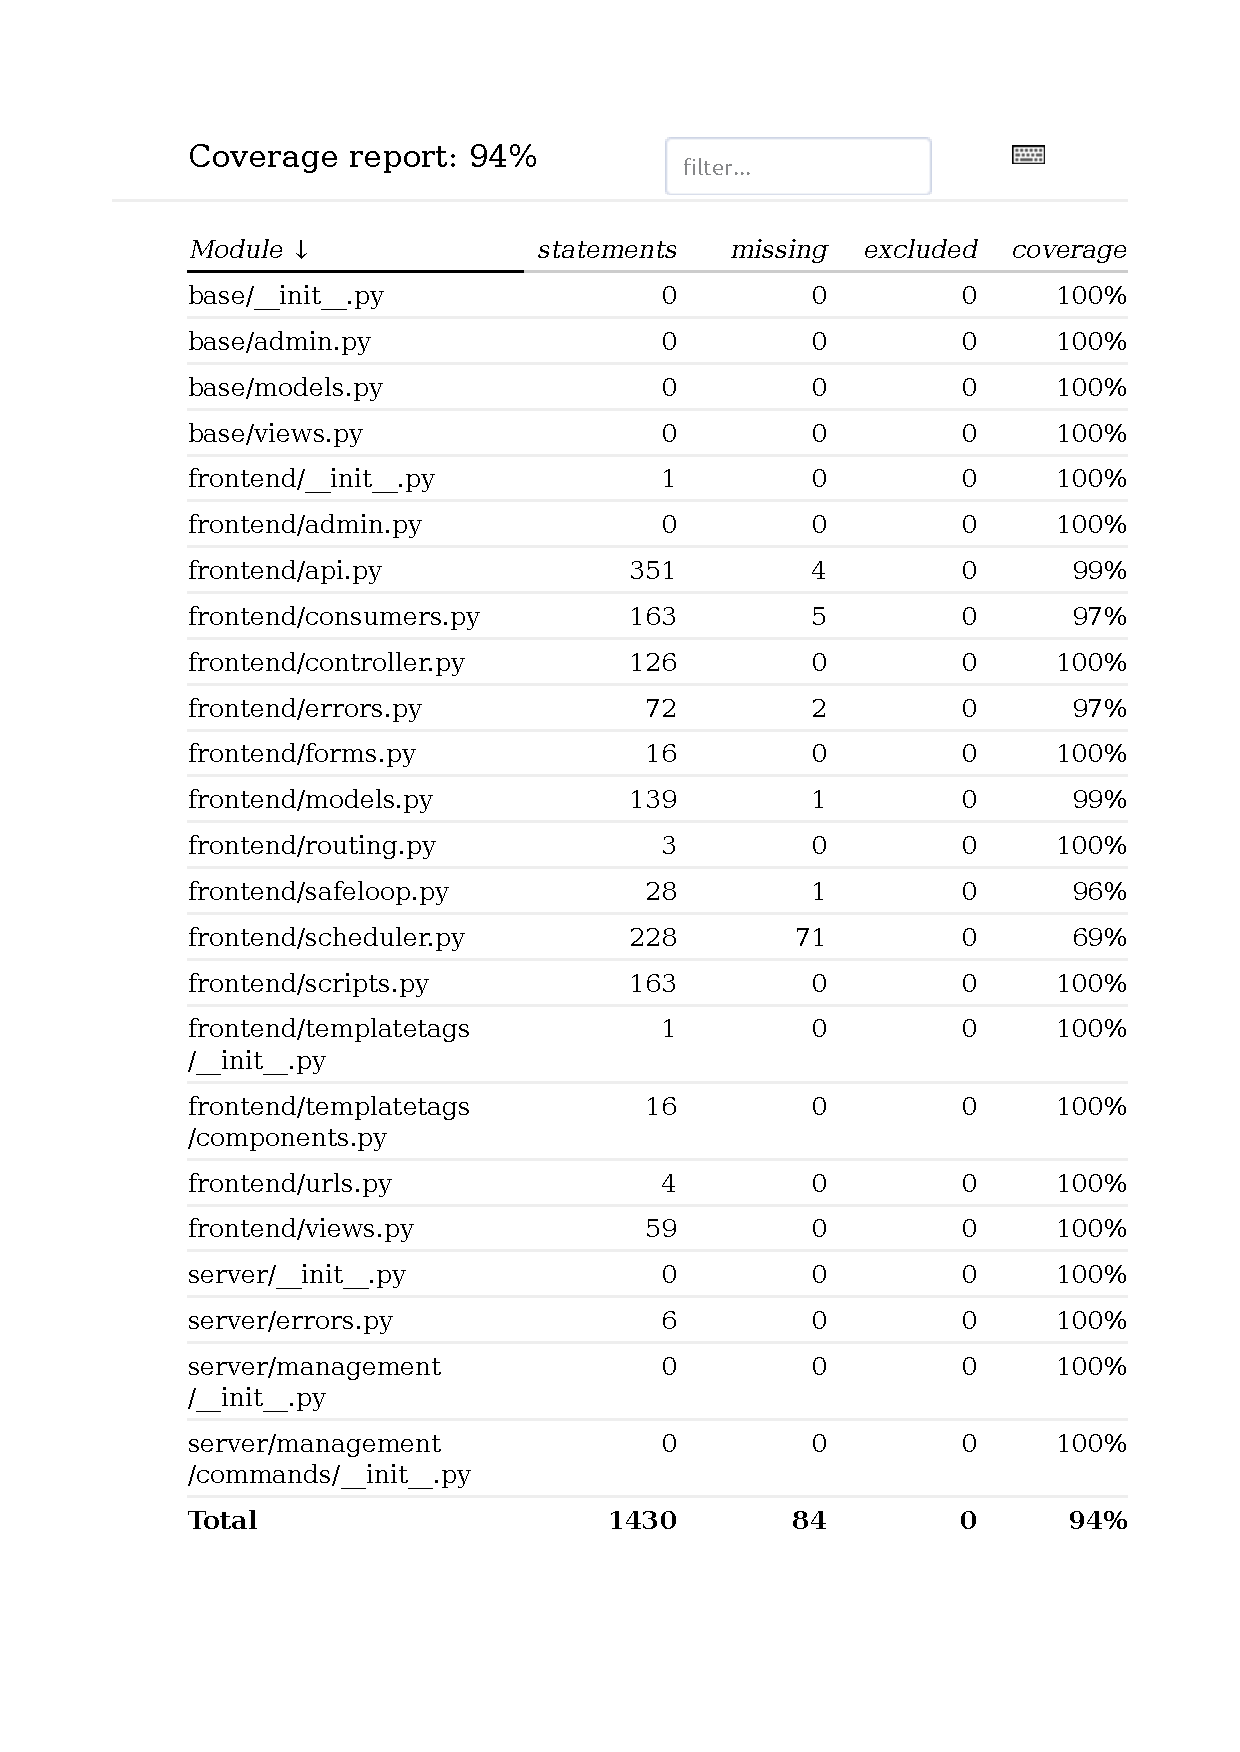
\includegraphics[width=.9\textwidth]{test_output/07_iteration_coverage.pdf}
	\caption{Coverage in Iteration 7}
\end{figure}

\subsubsection{8. Iteration}
\begin{table}[H]
\begin{center}
	\begin{tabular}{| l | l |}
		\hline
		\textbf{Zeitraum} &  05.03.2018 - 18.03.2018\\\hline
		\textbf{Abgegebene Userstorys} & 41, 45\\\hline
		\textbf{Commit Hash} & \texttt{13351d683a279c48b2890d23add9bfa57963fea8} \\\hline
	\end{tabular}
	\caption{Übersicht 8. Iteration}
\end{center}
\end{table}
\subsubsection{Testoutput }
\lstinputlisting{test_output/08_iteration_python}
\subsubsection{Coverage}
\begin{figure}[H]
	\centering
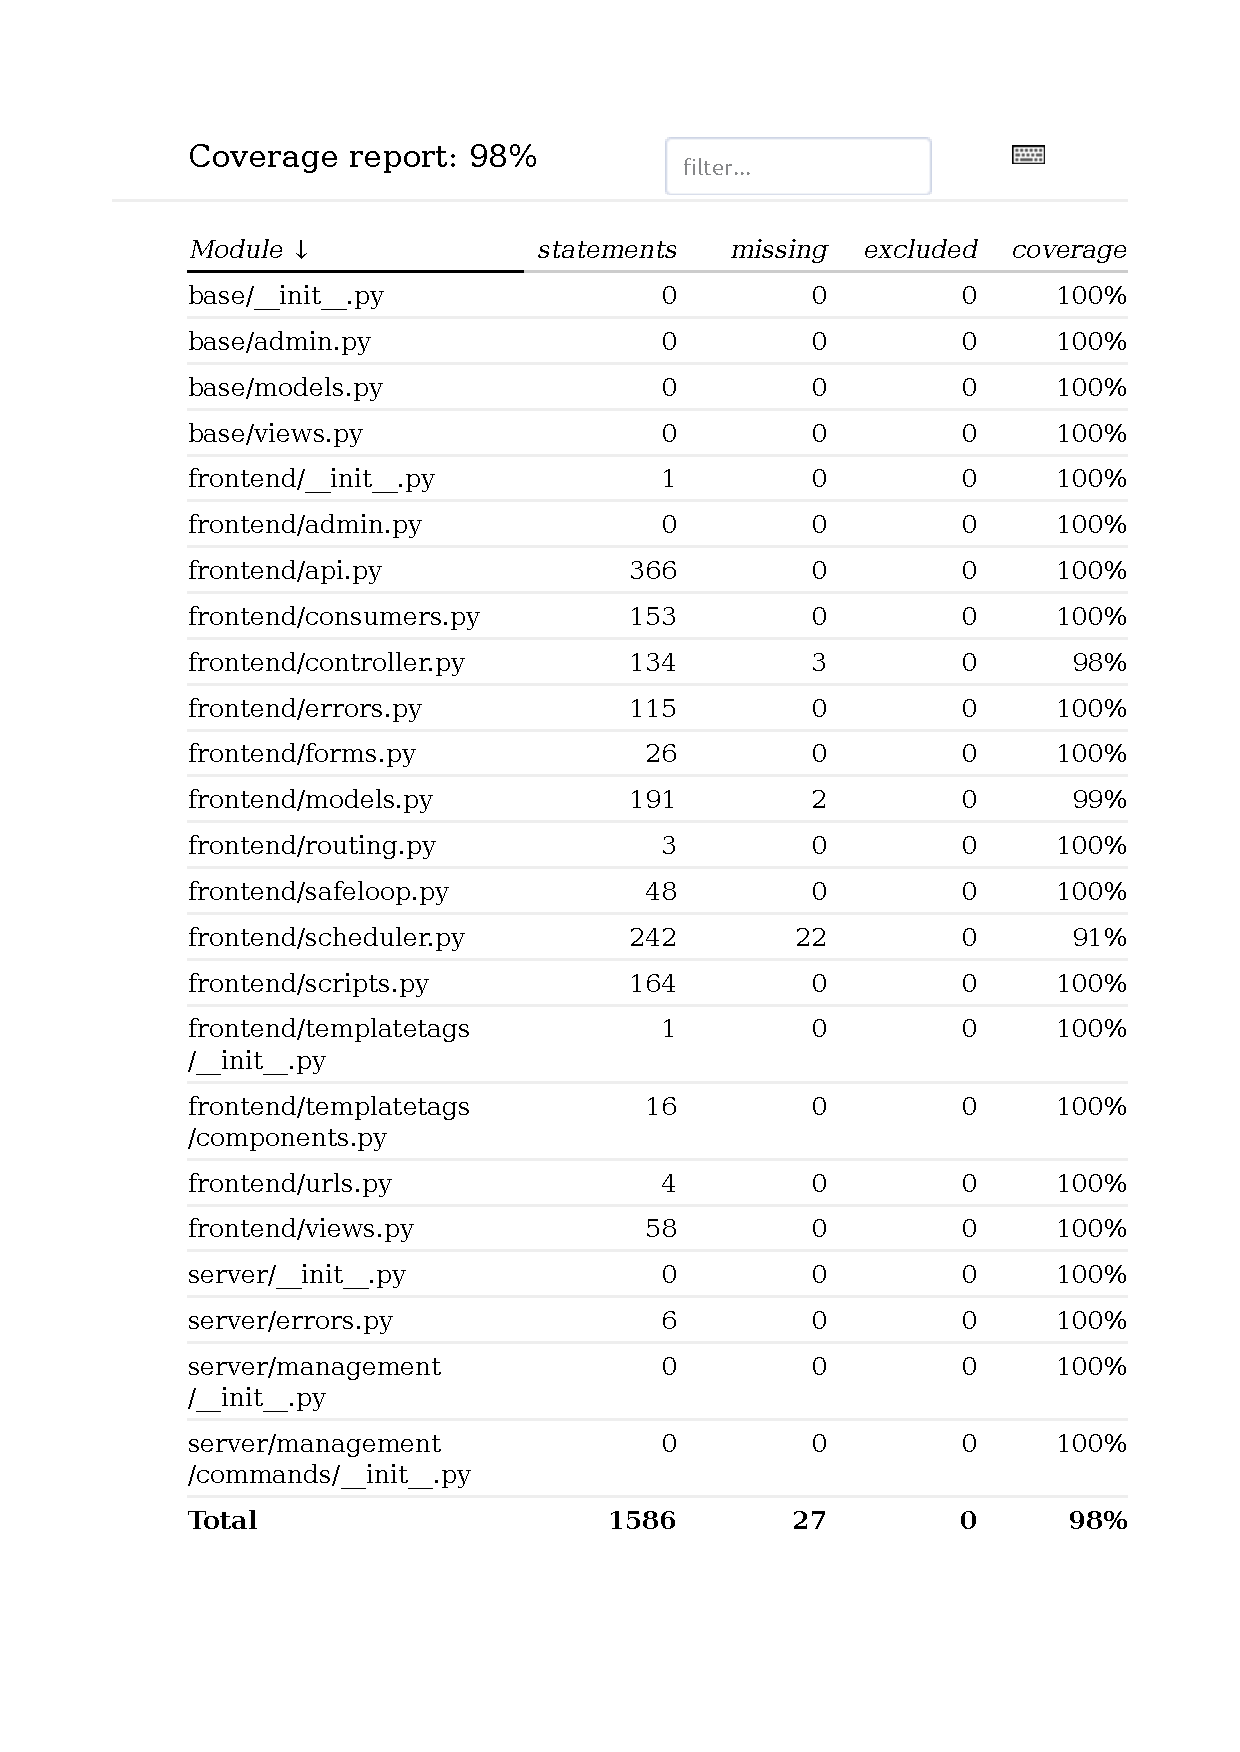
\includegraphics[width=.9\textwidth]{test_output/08_iteration_coverage.pdf}
	\caption{Coverage in Iteration 8}
\end{figure}

\subsubsection{9. Iteration}
\begin{table}[H]
\begin{center}
	\begin{tabular}{| l | l |}
		\hline
		\textbf{Zeitraum} &  19.03.2018 - 28.03.2018\\\hline
		\textbf{Abgegebene Userstorys} & 32, 42, 43, 44, 46, 47, 48\\\hline
		\textbf{Commit Hash} & \texttt{459b7edca36d0602017a1d724e2f159ce544aa1d} \\\hline
	\end{tabular}
	\caption{Übersicht 9. Iteration}
\end{center}
\end{table}
\subsubsection{Testoutput }
\lstinputlisting{test_output/09_iteration_python}
\subsubsection{Coverage}
\begin{figure}[H]
	\centering
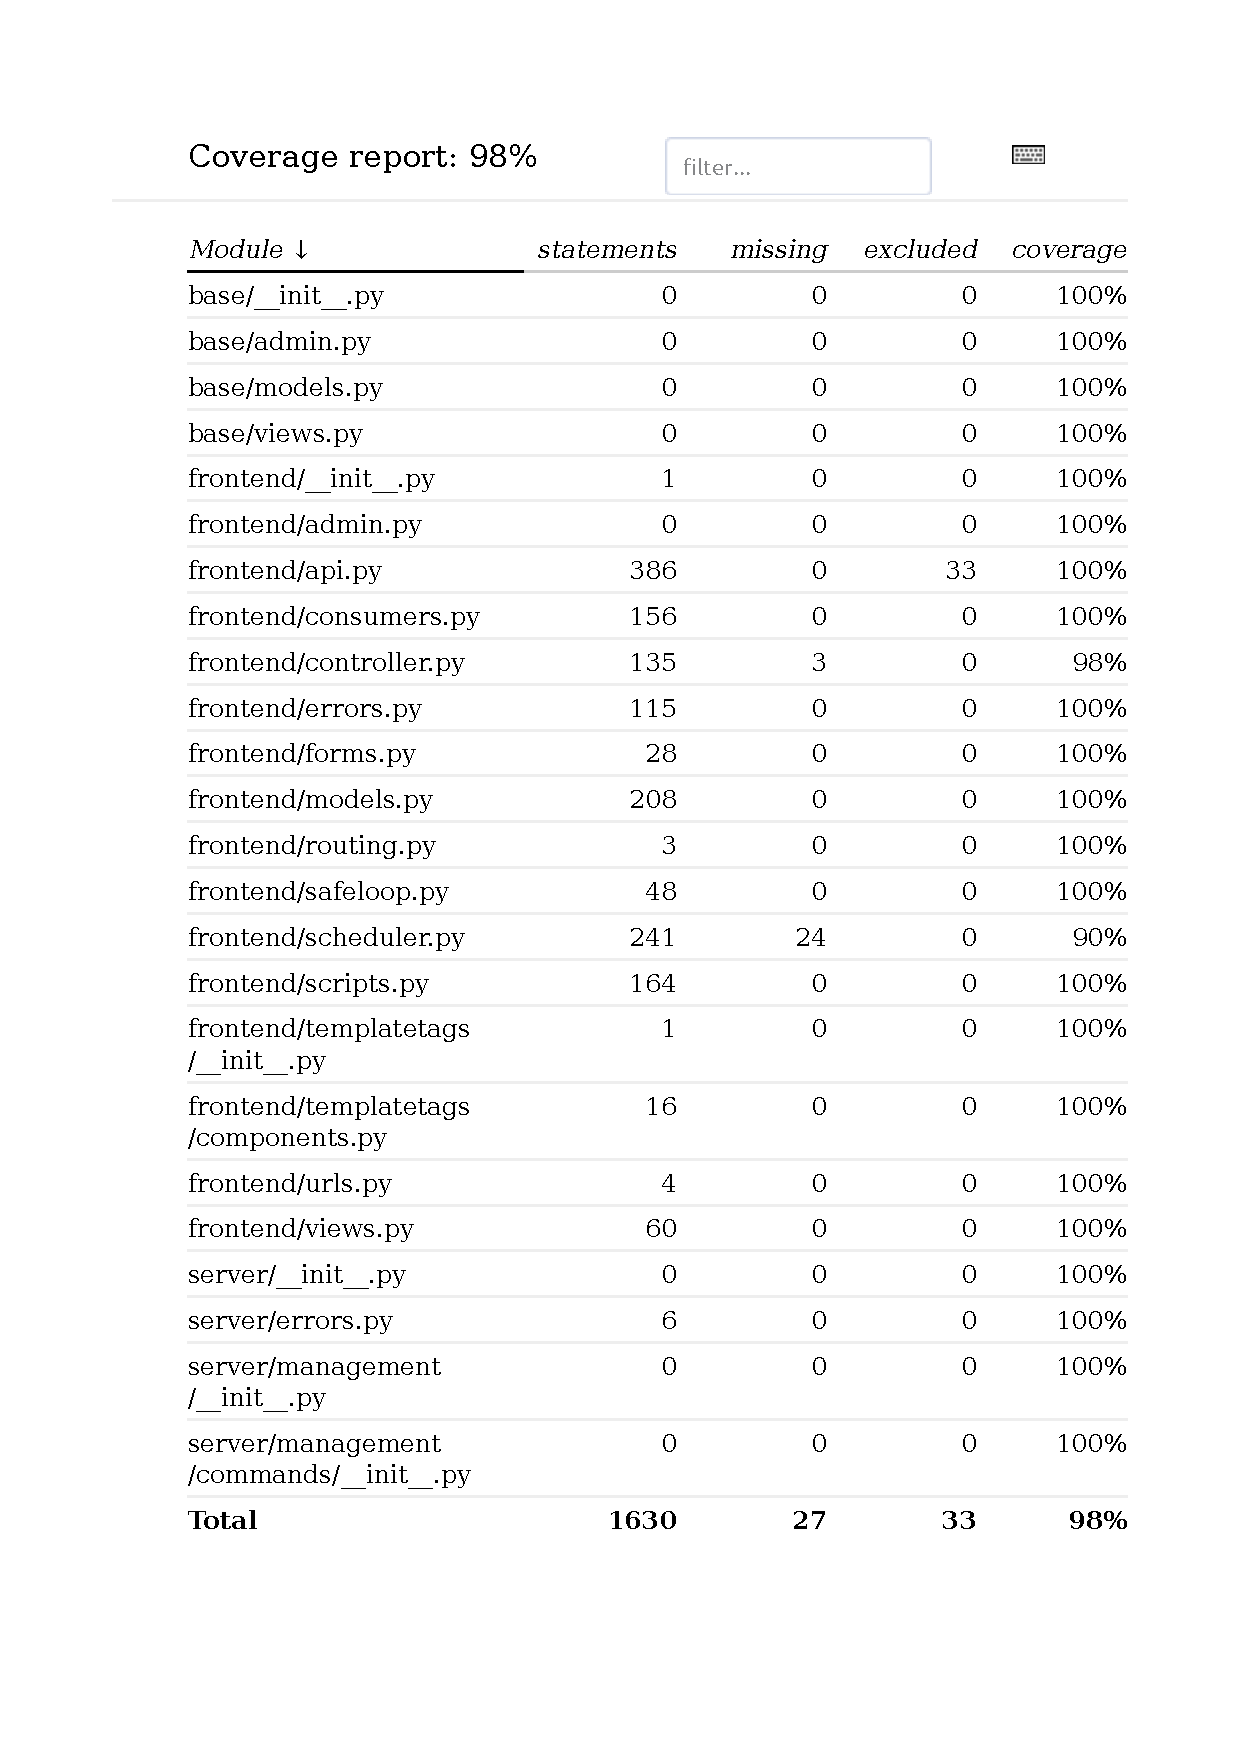
\includegraphics[width=.9\textwidth]{test_output/09_iteration_coverage.pdf}
	\caption{Coverage in Iteration 9}
\end{figure}
